\section{Proposed questions}
In this section, we answer point-to-point to the questions proposed during
project description.

\subsection{Describe the corpus $D$ and summaries $S$. Are terms uniformly distributed regarding TF-IDF?}
Fixed the x axis on terms, it can be seen by the figures that the plotted
distribution of words remains close to unchanged. However, it is important to
note that the y axis has a different scale, due to the smaller cardinality of
the summary set.
\begin{figure}[h]
    \centering
    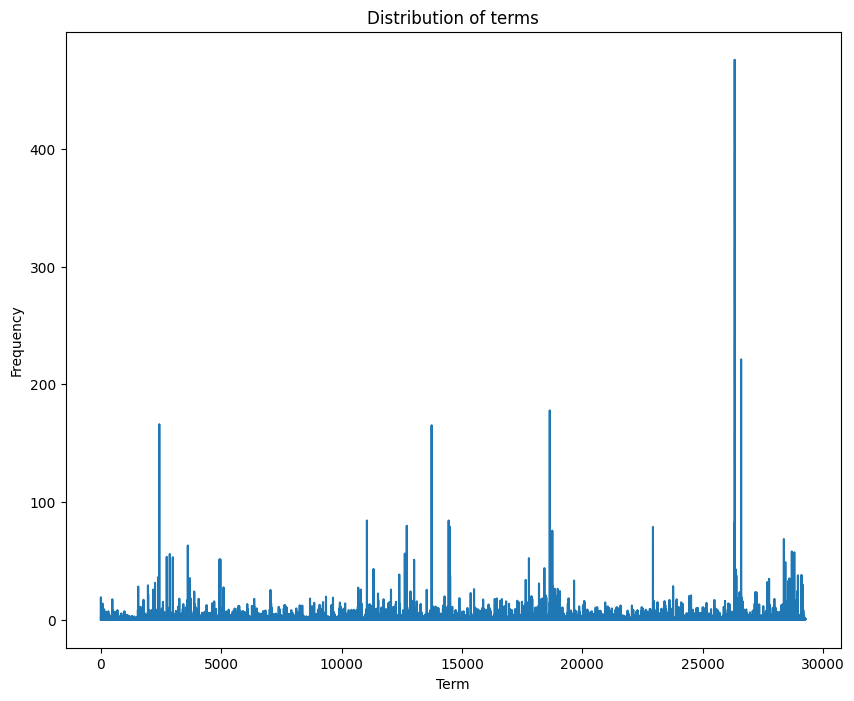
\includegraphics[width=0.45\textwidth]{images/dist_D.png}
    \caption{Corpus distribution}
    \label{fig:Corpus}
    \includegraphics*[width=0.45\textwidth]{images/dist_S.png}
    \caption{Summaries distribution}
    \label{fig:Summaries}
\end{figure}
\subsection{How does the summarization system perform for the full collection? And within each category? Any intuition for the observed differences?}
QUA SI POSSONO VEDERE DEI T TEST

Non mi trovo con il numero di sample. Da controllare

The following graph shows CONCLUSIONI

\begin{figure}[H]
    \centering
    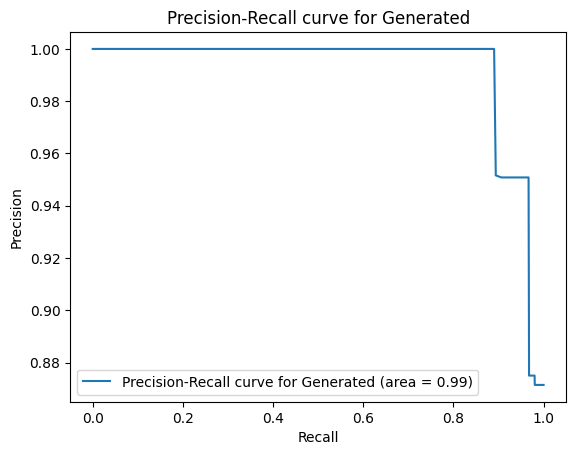
\includegraphics[width=0.7\textwidth]{images/whole_collection_performance.png}
    \caption{Performances}
    \label{fig:Performances}
\end{figure}

\begin{figure}[H]
    \centering
    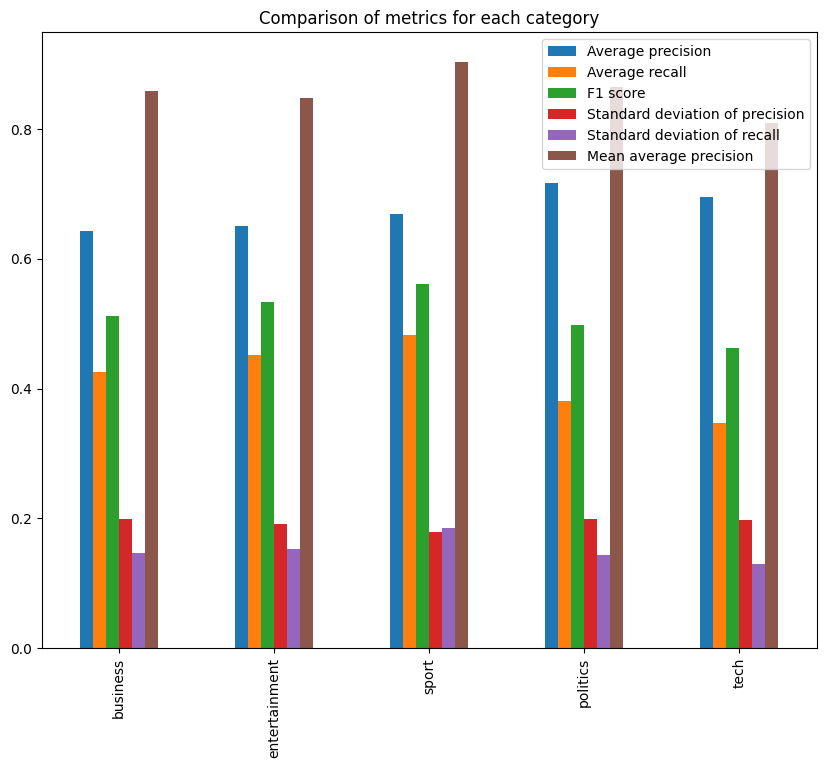
\includegraphics[width=0.7\textwidth]{images/class_comparison.png}
    \caption{Performances}
    \label{fig:Performances}
\end{figure}

\begin{center}
    \begin{table}[H]
        \centering
        \begin{tabular}{|l|c|c|c|c|c|}
            \hline
            Category          & Documents & Precision & Recall & F1    & MAP   \\
            \hline
            business          & 510       & 0.642     & 0.426  & 0.512 & 0.859 \\
            entertainment     & 386       & 0.651     & 0.452  & 0.533 & 0.848 \\
            sport             & 511       & 0.669     & 0.482  & 0.561 & 0.904 \\
            politics          & 417       & 0.717     & 0.381  & 0.498 & 0.864 \\
            tech              & 401       & 0.695     & 0.347  & 0.463 & 0.810 \\
            \hline
            whole\_collection & 2225      & 0.675     & 0.421  & 0.518 & 0.992 \\
            \hline
        \end{tabular}
        \caption{Performance metrics for different categories.}
        \label{tab:performance}
    \end{table}
\end{center}

\subsection{How IR models affect summaries? How vector space models compare with language models?}
Qua va un attimo contestualizzata la figura
\subsection{Is Reciprocal Rank Fusion (RRF) useful to aid decisions?}
We expected that RRF would help to improve the summaries, since it's a way to
combine the results of different systems and, in machine learning contexts,
ensembles are generally outperforming single models. \\ Our test was not done
on the entire collection due to the scarcity of computational power. Thus, we
conduced a test on a subset of the dataset,that didn't really show any
particular improvement on the scoring metrics. Due to this, we can say that RRF
did not improve our system, but we cannot say that in general, since the size
of our testing dataset was not significative and the BERT implementation is
based on our suppositions. Moreover, a BERT-based solution is not suggested
since the model usage times, combined with the additional overhead caused by
calculating distances in the latent space, cause a significant slower response.


\begin{center}
    \begin{table}[H]
        \centering
        \begin{tabular}{|l|c|c|c|c|c|c|}
            \hline
            Method & Avg. Prec & Avg. Rec & F1 Score & Std Prec & Std Rec & MAP    \\
            \hline
            BM25   & 0.7554    & 0.4250   & 0.5440   & 0.1962   & 0.1574  & 0.7869 \\
            \hline
            RRF    & 0.5105    & 0.2832   & 0.3643   & 0.1223   & 0.1140  & 0.5014 \\
            \hline
        \end{tabular}
        \caption{Performance metrics for BM25 and RRF.}
        \label{tab:bm25_rrf}
    \end{table}
\end{center}

\subsection{Considering MMR, how $\lambda$ impacts the accuracy (against ideal extracts) of summaries? Should $\lambda$ be a fixed threshold or depend on the provided topic document (d-specific)?}
Qua la figura va rivista, le lambda nell'asse x non corrispondono ai valori
proposti e poi l'asse sembra su un insieme continuo. Ho provato a leggere il
codice, non capisco che sta facendo
\subsection{At the suggested $p$ length threshold, is the system better at promoting recall or precision?}

? che stai provando a dire? \\Every time we try to measure the performance of a system, we always see that the precision is the higest, but the recall is the lowest. This is because the system is trying to avoid to put in the summary a sentence that is not relevant, but this can lead to a lower recall.

\begin{figure}
    \centering
    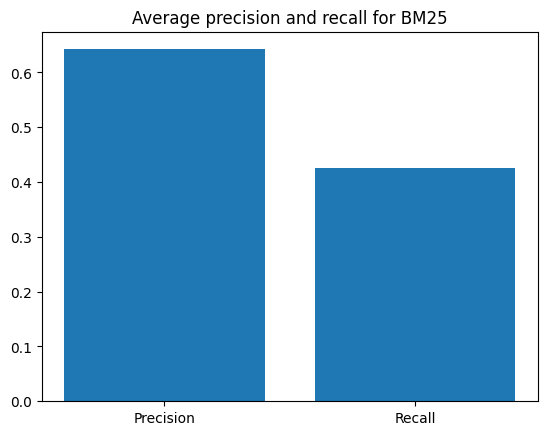
\includegraphics[width=0.9\textwidth]{images/pre_rec.png}
    \caption{Precision and recall at given threshold}
    \label{fig:Precision and recall}
\end{figure}